
\section{RAMP Transaction Algorithms}
\label{sec:ramp-algorithm}

Given specifications for RA isolation and scalability, we present
algorithms for achieving both. For ease of understanding, we first
focus on providing read-only and write-only transactions with a ``last
writer wins'' overwrite policy, then subsequently discuss how to
perform read/write transactions. Our focus in this section is on
intuition and understanding; we defer all correctness and scalability
proofs to Section~\ref{sec:rampproofs}, providing salient details inline.

At a high level, RAMP transactions allow reads and writes to proceed
concurrently. This provides excellent performance but, in turn,
introduces certain race conditions that could cause undesirable
anomalies: one transaction might only read a subset of another
transaction's writes, violating RA (i.e., fractured reads might
occur). Instead of preventing this race (hampering scalability), RAMP
readers \textit{autonomously} detect the race (using metadata attached
to each data item) and fetch any missing, in-flight writes from their
respective partitions. To make sure that readers never have to wait
for writes to arrive at a partition, writers use a two-phase (atomic
commitment) protocol that ensures that once a write is visible to
readers on one partition, any other writes in the transaction are
present on and, if appropriately identified by version, readable from
their respective partitions.

In this section, we present three algorithms that provide a trade-off
between the amount of metadata required and the expected number of
extra reads to fetch missing writes. As discussed in
Section~\ref{sec:motivation}, while techniques like distributed
locking couple mutual exclusion with atomic visibility of writes, RAMP
transactions correctly control visibility but allow concurrent and
scalable execution.

\subsection{RAMP-Fast}
\label{sec:rapl}


\begin{figure}[t!]
\begin{center}
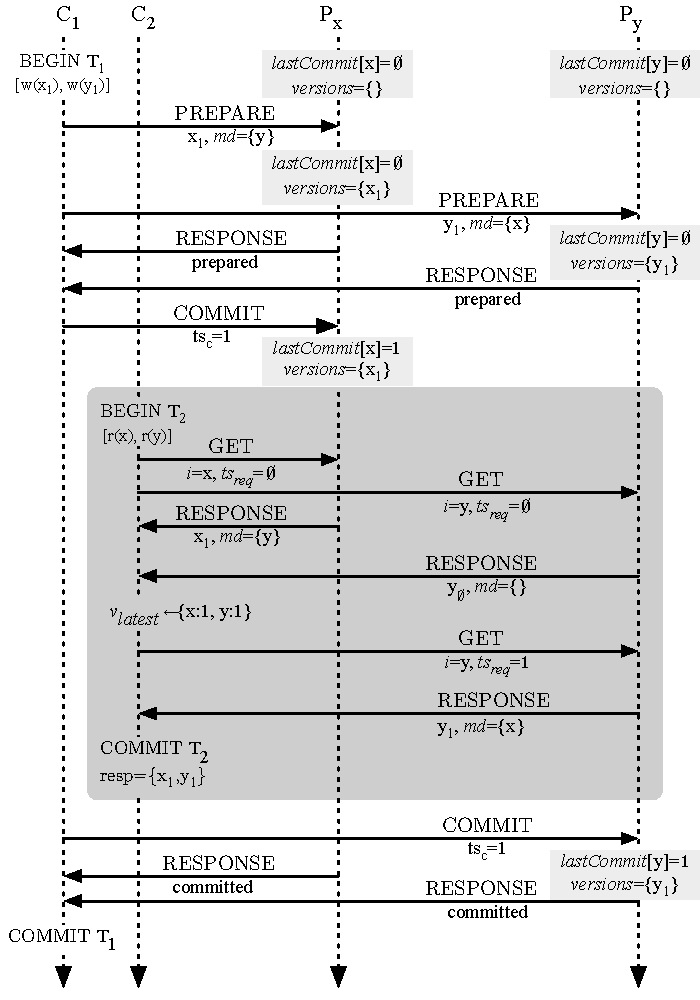
\includegraphics[width=.6\columnwidth]{diagram/rapl-big.pdf}\vspace{.5em}
\caption{Space-time diagram for \rapl execution for two transactions
  $T_1$ and $T_2$ performed by clients $C_1$ and $C_2$ on partitions
  $P_x$ and $P_y$. Lightly-shaded boxes represent current partition
  state ($lastCommit$ and $versions$), while the single darker box
  encapsulates all messages exchanged during $C_2$'s execution of
  transaction $T_2$.  Because $T_1$ overlaps with $T_2$, $T_2$ must
  perform a second round of reads to repair the fractured read between
  $x$ and $y$. $T_1$'s writes are assigned timestamp $1$. In our
  depiction, each item does not appear in its list of writes (e.g.,
  $P_x$ sees $\{y\}$ only and not $\{x,y\}$.}
\label{fig:rapl-execution}
\end{center}
\end{figure}

To begin, we present a RAMP algorithm that, in the race-free case,
requires one RTT for reads and two RTTs for writes, called
\texttt{RAMP-Fast} (abbreviated \rapl; Algorithm~\ref{alg:rapl}).
\rapl stores metadata in the form of write sets (overhead linear in
transaction size).

\minihead{Overview} Each write in \rapl
(lines~\ref{rapl-putall-start}--\ref{rapl-putall-end}) contains a
timestamp (line~\ref{rapl-newid}) that uniquely identifies the writing
transaction as well as a set of items written in the transaction
(line~\ref{rapl-metadata}). For now, combining a unique client ID and
client-local sequence number is sufficient for timestamp generation
(see also Section~\ref{sec:additional}).

\rapl write transactions proceed in two phases: a first round of
communication places each timestamped write on its respective
partition. In this \textsc{prepare} phase, each partition adds the
write to its local database ($versions$,
lines~\ref{rapl-versions},~\ref{rapl-beginprepare-client}--\ref{rapl-endprepare-client}). A
second round of communication
(lines~\ref{rapl-begincommit-client}--\ref{rapl-endcommit-client}) marks versions as committed. In this
\textsc{commit} phase, each partition updates an index containing the
highest-timestamped committed version of each item ($lastCommit$,
lines~\ref{rapl-lc},~\ref{rapl-begincommit-server}--\ref{rapl-endcommit-server}).

\rapl read transactions begin by first fetching the last
(highest-timestamped) committed version for each item from its
respective partition
(lines~\ref{rapl-client-firstround-start}--\ref{rapl-client-secondround-start}). Using
the results from this first round of reads, each reader can calculate
whether it is ``missing'' any versions (that is, versions that were
prepared but not yet committed on their partitions). The reader
calculates a mapping from each item $i$ to the highest timestamped
version of $i$ that appears in the metadata of any version (of $i$ or
of any other item) in the first-round read set
(lines~\ref{rapl-client-latest-start}--\ref{rapl-client-latest-end}). If
the reader has read a version of an item that has a lower timestamp
than indicated in the mapping for that item, the reader issues a
second read to fetch the missing version (by timestamp) from its
partition
(lines~\ref{rapl-client-secondround-start}--\ref{rapl-client-secondround-end}). Once
all missing versions are fetched (which can be done in parallel), the
client can return the resulting set of versions---the first-round
reads, with any missing versions replaced by the optional, second
round of reads.

\minihead{By example} Consider the \rapl execution depicted in
Figure~\ref{fig:rapl-execution}. $T_1$ writes to both $x$ and $y$,
performing the two-round write protocol on two partitions, $P_x$ and
$P_y$. However, $T_2$ reads from $x$ and $y$ while $T_1$ is
concurrently writing.  Specifically, $T_2$ reads from $P_x$
\textit{after} $P_x$ has committed $T_1$'s write to $x$, but $T_2$
reads from $P_y$ \textit{before} $P_y$ has committed $T_1$'s write to
$y$. Therefore, $T_2$'s first-round reads return $x=x_1$ and $y=\bot$,
and returning this set of reads would violate RA. Using the metadata
attached to its first-round reads, $T_2$ determines that it is missing
$y_1$ (since $v_{latest}[y]=1$ and $1 > \bot$) and so $T_2$
subsequently issues a second read from $P_y$ to fetch $y_1$ by
version. After completing its second-round read, $T_2$ can safely
return its result set. $T_1$'s progress is unaffected by $T_2$, and
$T_1$ subsequently completes by committing $y_1$ on $P_y$.



\minihead{Why it works} \rapl writers use metadata as a record of
intent: a reader can detect if it has raced with an in-progress commit
round and use the metadata stored by the writer to fetch the missing
data. Accordingly, \rapl readers only issue a second round of reads in
the event that they read from a partially-committed write transaction
(where some but not all partitions have committed a write). In this
event, readers will fetch the appropriate writes from the
not-yet-committed partitions. Most importantly, \rapl readers never
have to stall waiting for a write that has not yet arrived at a
partition: the two-round \rapl write protocol guarantees that, if a
partition commits a write, all of the corresponding writes in the
transaction are present on their respective partitions (though
possibly not committed locally). As long as a reader can identify the
corresponding version by timestamp, the reader can fetch the version
from the respective partition's set of pending writes without
waiting. To enable this, \rapl writes contain metadata linear in the
size of the writing transaction's write set (plus a timestamp per
write).\vspace{.5em}

\rapl requires two RTTs for writes: one for \textsc{prepare}
and one for \textsc{commit}. For reads, \rapl requires one RTT in the
absence of concurrent writes and two RTTs otherwise.

RAMP timestamps are only used to identify specific versions and in
ordering concurrent writes to the same item; \rapl transactions do not
require a ``global'' timestamp authority. For example, if
$lastCommit[k]=2$, there is no requirement that a transaction
with timestamp $1$ has committed or even that such a transaction
exists.

\begin{algorithm}[t!]
\small
\caption{RAMP-Fast}
\label{alg:rapl}
\newcommand{\myindent}{\hspace{-1em}}

\begin{algorithmic}[1]
\Statex{\textbf{\textit{Server-side Data Structures}}\\
$versions$: set of versions $\langle item, value,$ timestamp $ts_v,$ metadata $md\rangle$ \label{rapl-versions}\\
$lastCommit[i]$: last committed timestamp for item $i$\label{rapl-lc}}\vspace{.5em}

\Statex{\textbf{\textit{Server-side Methods}}}\vspace{.25em}

\Procedure{prepare}{$v$ : version}\label{rapl-beginprepare-server}
  \State $versions$.add($v$)\label{rapl-server-prepare}
  \State \Return
\EndProcedure\vspace{.5em}\label{rapl-endprepare-server}

\Procedure{commit}{$ts_c$ : timestamp}\label{rapl-begincommit-server}
  \State $I_{ts} \gets$ $\{w.item \mid w \in versions \wedge w.ts_v = ts_c\}$\label{rapl-server-commit-1}
  \State $\forall i \in I_{ts}$, $lastCommit[i] \gets
  \max(lastCommit[i], ts_c)$\label{rapl-server-commit-2}
\EndProcedure\vspace{.5em}\label{rapl-endcommit-server}

\Procedure{get}{$i$ : item, $ts_{req}$ : timestamp}\label{rapl-get-server-start}
  \If {$ts_{req} = \emptyset$\label{rapl-get-server-nots-start}}
  \State {\Return $v \in versions : v.item=i \wedge v.ts_v = lastCommit[item]$\label{rapl-get-server-nots-end}}
  \Else 
  \State {\Return $v \in versions : v.item = i \wedge  v.ts_v = ts_{req}$\label{rapl-get-server-withts-end}}
  \EndIf
\EndProcedure\label{rapl-get-server-end}
\Statex\hrulefill\vspace{.25em}

\Statex{\textbf{\textit{Client-side Methods}}}\vspace{.25em}

\Procedure{put\_all}{$W$ : set of $\langle item, value \rangle$}\label{rapl-putall-start}
  \State $ts_{tx} \gets$ generate new timestamp\label{rapl-newid}
  \State $I_{tx} \gets $ set of items in $W$\label{rapl-metadata}
  \ParFor{$\langle i, v\rangle \in W$}\label{rapl-beginprepare-client}
  \State $v \gets \langle item=i, value=v, ts_v=ts_{tx}, md=(I_{tx} - \{i\})\rangle$\label{rapl-prepare-data}
  \State\hspace{1em} invoke $\textsc{prepare}(v)$ on respective server (i.e., partition)\label{rapl-prepare-client}
  \EndParFor\label{rapl-endprepare-client}
  
  \ParFor{server $s : s$ contains an item in $W$}\label{rapl-begincommit-client}
  \State invoke $\textsc{commit}(ts_{tx})$ on $s$\label{rapl-commit-client}
  \EndParFor\label{rapl-endcommit-client}
\EndProcedure\vspace{.5em}\label{rapl-putall-end}

\Procedure{get\_all}{$I$ : set of items}\label{rapl-client-getall-start}
  \State $ret \gets \{\}$\label{rapl-client-firstround-start}
  \ParFor {$i \in I$}
  \State $ret[i] \gets \textsc{get}(i, \emptyset)$\label{rapl-client-firstround-get}
  \EndParFor\vspace{.25em}\label{rapl-client-firstround-end}

  \State $v_{latest} \gets \{\}$ (default value: $-1$)\label{rapl-client-latest-start}
  \For{response $r \in ret$}
  \For{$i_{tx} \in r.md$}
  \State $v_{latest}[i_{tx}] \gets \max(v_{latest}[i_{tx}], r.ts_v)$\label{rapl-client-latest-calculate}
  \EndFor
  \EndFor\vspace{.25em}\label{rapl-client-latest-end}

  \ParFor{item $i \in I$}\label{rapl-client-secondround-start}
  \If{$v_{latest}[i] > ret[i].ts_v$}\label{rapl-client-secondround-check}
  \State $ret[i] \gets \textsc{get}(i, v_{latest}[i])$\label{rapl-client-secondround-get}
  \EndIf
  \EndParFor\vspace{.25em}\label{rapl-client-secondround-end}

  \State \Return $ret$\label{rapl-client-getall-return}
\EndProcedure\label{rapl-client-getall-end}


\end{algorithmic}
\end{algorithm}


\subsection{RAMP-Small: Trading Metadata for RTTs}
\label{sec:raps}

\begin{figure}[t!]
\begin{center}
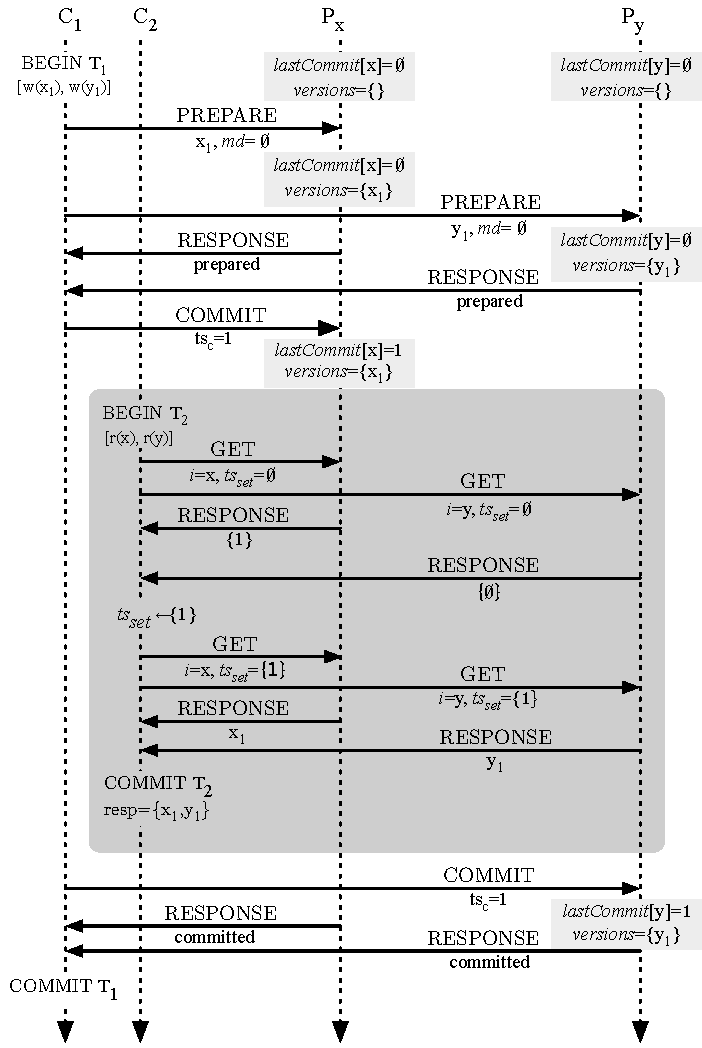
\includegraphics[width=.6\columnwidth]{diagram/raps-big.pdf}\vspace{.5em}
\caption{Space-time diagram for \raps execution for two transactions
  $T_1$ and $T_2$ performed by clients $C_1$ and $C_2$ on partitions
  $P_x$ and $P_y$. Lightly-shaded boxes represent current partition
  state ($lastCommit$ and $versions$), while the single darker box
  encapsulates all messages exchanged during $C_2$'s execution of
  transaction $T_2$. $T_1$ first fetches the highest committed
  timestamp from each partition, then fetches the corresponding
  version. In this depiction, partitions only return timestamps
  instead of actual versions in response to first-round reads.}
\label{fig:raps-execution}
\end{center}
\end{figure}

While \rapl requires metadata size linear in write set size but provides best-case
one RTT for reads, \texttt{RAMP-Small} (\raps) uses constant
metadata but always requires two RTT for reads
(Algorithm~\ref{alg:raps}). \raps and \rapl writes are identical, but,
instead of attaching the entire write set to each write, \raps writers
only store the transaction timestamp
(line~\ref{raps-prepare-data}). Unlike \rapl, \raps readers issue a
first round of reads to fetch the highest committed timestamp for each
item from its respective partition
(lines~\ref{raps-get-server-nots-end},~\ref{raps-client-firstround-start}--\ref{raps-client-firstround-end}). Then
the readers send the entire set of timestamps they received to
the partitions in a second round of communication
(lines~\ref{raps-client-secondround-start}--\ref{raps-client-secondround-end}). For
each item in the read request, \raps servers return the
highest-timestamped version of the item that also appears in the
supplied set of timestamps
(lines~\ref{raps-get-server-withts-start}--\ref{raps-get-server-withts-end}). Readers
subsequently return the results from the mandatory second round of
requests.

\minihead{By example} In Figure~\ref{fig:raps-execution}, under \raps,
$P_x$ and $P_y$ respectively return the sets $\{1\}$ and
$\{\bot\}$ in response to $T_2$'s first round of reads. $T_2$ would
subsequently send the set $\{1, \bot\}$ to both $P_x$ and $P_y$, which
would return $x_1$ and $y_1$.  (Including $\bot$ in the second-round
request is unnecessary, but we leave it in for ease of understanding.)

\minihead{Why it works} In \raps, if a transaction has committed on
some but not all partitions, the transaction timestamp will be
returned in the first round of any concurrent read transaction
accessing the committed partitions' items. In the (required) second
round of read requests, any prepared-but-not-committed partitions will
find the committed timestamp in the reader-provided set and return the
appropriate version. In contrast with \rapl, where readers explicitly
provide partitions with a specific version to return in the (optional)
second round, \raps readers defer the decision of which version to
return to the partition, which uses the reader-provided set to
decide. This saves metadata but increases RTTs, and the size of the
parameters of each second-round \textsc{get} request is (worst-case)
linear in the read set size. Unlike \rapl, there is no requirement to
return the value of the last committed version in the first round
(returning the version, $lastCommit[k]$, suffices in
line~\ref{raps-get-server-nots-end}).

\begin{algorithm}[t!]
\small
\caption{RAMP-Small}
\label{alg:raps}
\newcommand{\myindent}{\hspace{-1em}}
\begin{algorithmic}[1]
\Statex{\textbf{\textit{Server-side Data Structures}}}
\Statex same as in \rapl (Algorithm~\ref{alg:rapl}) \vspace{.5em}

\Statex{\textbf{\textit{Server-side Methods}}}\
\Statex \textsc{prepare}, \textsc{commit} same as in \rapl\vspace{.5em}

\Procedure{get}{$i$ : item, $ts_{set}$ : set of timestamps}\label{raps-get-server-start}
  \If{$ts_{set} = \emptyset$}
  \State \Return $v \in versions : v.item=i \wedge v.ts_v =
  lastCommit[k]$\label{raps-get-server-nots-end}
  \Else
  \State $ts_{match} = \{t \mid t \in ts_{set} \wedge \exists v \in versions : v.item = i \wedge v.t_v = t\}$\label{raps-get-server-withts-start}
  \State \Return $v \in versions : v.item = i \wedge  v.ts_v =
  max(ts_{match})$\label{raps-get-server-withts-end}
  \EndIf

\EndProcedure\label{raps-get-server-end}
\Statex\hrulefill\vspace{.25em}

\Statex{\textbf{\textit{Client-side Methods}}}\vspace{.25em}

\Procedure{put\_all}{$W$ : set of $\langle item, value \rangle$}
\Statex \hspace{1.5em} same as \rapl \textsc{put\_all} but do not instantiate $md$ on line~\ref{rapl-prepare-data}\label{raps-prepare-data}
\EndProcedure\vspace{.5em}\label{raps-putall-end}

\Procedure{get\_all}{$I$ : set of items}\label{raps-client-getall-start}
\State \hspace{.35em} $ts_{set} \gets \{\}$\label{raps-client-firstround-start}
\ParFor {$i \in I$}
    \State $ts_{set}.$add($\textsc{get}(i, \emptyset).ts_v$)\label{raps-client-firstround-get}
  \EndParFor\vspace{.25em}\label{raps-client-firstround-end}

  \State $ret \gets \{\}$
  \ParFor{item $i \in I$}\label{raps-client-secondround-start}
    \State $ret[i] \gets \textsc{get}(i, ts_{set})$ \label{raps-client-secondround-get}
  \EndParFor\vspace{.25em}\label{raps-client-secondround-end}

  \State \Return $ret$\label{raps-client-getall-return}
\EndProcedure\label{raps-client-getall-end}


\end{algorithmic}
\end{algorithm}

\subsection{RAMP-Hybrid: An Intermediate Solution}
\label{sec:rapb}

\texttt{RAMP-Hybrid} (\rapb; Algorithm~\ref{alg:rapb}) strikes a
compromise between \rapl and \raps. \rapb and \raps write protocols
are identical, but, instead of storing the entire write set (as in
\rapl), \rapb writers store a Bloom filter~\cite{bloomfilter}
representing the transaction write set
(line~\ref{rapb-putall-start}). \rapb readers proceed as in \rapl, with
a first round of communication to fetch the last-committed version of
each item from its partition
(lines~\ref{rapb-client-firstround-start}--\ref{rapb-client-firstround-end}). Given
this set of versions, \rapb readers subsequently compute a list of
\textit{potentially} higher-timestamped writes for each item
(lines~\ref{rapb-client-compute-start}--\ref{rapb-client-compute-end}). Any
potentially missing versions are fetched in a second round of reads
(lines~\ref{rapb-client-secondround-start}).

\minihead{By example} In Figure~\ref{fig:rapl-execution}, under \rapb,
$x_1$ would
contain a Bloom filter with positives for $x$ and $y$ and $y_{\bot}$
would contain an empty Bloom filter. $T_2$ would check for the
presence of $y$ in $x_1$'s Bloom filter (since $x_1$'s version is $1$
and $1 > \bot$) and, finding a match, conclude that it is potentially
missing a write ($y_1$). $T_2$ would subsequently fetch $y_1$ from
$P_y$.

\minihead{Why it works} \rapb is effectively a hybrid between \rapl
and \raps. If the Bloom filter has no false positives, \rapb reads
behave like \rapl reads. If the Bloom filter has all false positives,
\rapb reads behave like \raps reads. Accordingly, the number of
(unnecessary) second-round reads (i.e., which would not be performed
by \rapl) is controlled by the Bloom filter false positive rate, which
is in turn (in expectation) proportional to the size of the Bloom
filter. Any second-round \textsc{get} requests are accompanied by a
set of timestamps that is also proportional in size to the false
positive rate.  Therefore, \rapb exposes a trade-off between metadata
size and expected performance. To understand why \rapb is safe, we
simply have to show that any false positives (second-round reads) will
not compromise the integrity of the result set; with unique
timestamps, any reads due to false positives will return null.

\begin{algorithm}[t!]
\small
\caption{RAMP-Hybrid}
\label{alg:rapb}
\newcommand{\myindent}{\hspace{-1em}}
\begin{algorithmic}[1]
\Statex{\textbf{\textit{Server-side Data Structures}}}
\Statex same as in \rapl (Algorithm~\ref{alg:rapl}) \vspace{.5em}

\Statex{\textbf{\textit{Server-side Methods}}}\
\Statex \textsc{prepare}, \textsc{commit} same as in \rapl
\Statex \textsc{get} same as in \raps
\Statex\hrulefill\vspace{.25em}

\Statex{\textbf{\textit{Client-side Methods}}}\vspace{.25em}

\Procedure{put\_all}{$W$ : set of $\langle item, value \rangle$}~\label{rapb-putall-start}
\Statex \hspace{1.5em} same as \rapl \textsc{put\_all} but instantiate $md$ on line~\ref{rapl-prepare-data}
\Statex \hspace{1.5em} with Bloom filter containing $I_{tx}$
\EndProcedure\vspace{.5em}\label{rapb-putall-end}

\Procedure{get\_all}{$I$ : set of items}\label{rapb-client-getall-start}
  \State $ret \gets \{\}$\label{rapb-client-firstround-start}
  \ParFor {$i \in I$}
  \State $ret[i] \gets \textsc{get}(i, \emptyset)$\label{rapb-client-firstround-get}
  \EndParFor\vspace{.25em}\label{rapb-client-firstround-end}

  \State $v_{fetch} \gets \{\}$

  \For{version $v \in ret$}\label{rapb-client-compute-start}
  \For{version $v' \in ret: v' \neq v$}
  \If{$v.ts_v > v'.ts_v \wedge v.md.lookup(v'.item) \rightarrow True$}
    \State $v_{fetch}[v'.item]$.add($v.ts_v$)\label{rapb-client-compute-step}
  \EndIf
  \EndFor
  \EndFor\label{rapb-client-compute-end}

  \ParFor{item $i \in v_{fetch}$}\label{rapb-client-secondround-start}
        \State $ret[i] \gets \textsc{get}(k, v_{fetch}[i])$ \textbf{if}
        $\textsc{get}(k, v_{fetch}[i]) \neq \bot$ \label{rapb-client-secondround-get}
  \EndParFor\vspace{.25em}\label{rapb-client-secondround-start}
  \State \Return $ret$\label{rapb-client-getall-return}
\EndProcedure\label{rapb-client-getall-end}


\end{algorithmic}
\end{algorithm}


\subsection{Summary and Additional Details}

The RAMP algorithms allow readers to safely race writers without
requiring either to stall. The metadata attached to each write allows
readers in all three algorithms to safely handle concurrent and/or
partial writes and in turn allows a trade-off between metadata size
and performance (Table~\ref{table:rap-compare}): \rapl is optimized
for fast reads, \raps is optimized for small metadata, and \rapb is,
as the name suggests, a middle ground. \rapl requires metadata linear
in transaction size, while \raps and \rapb require constant
metadata. However, \raps and \rapb require more RTTs for reads
compared to \rapl when there is no race between readers and
writers. When reads and writes race, in the worst case, all algorithms
require two RTTs for reads.  Writes always require two RTTs to prevent
readers from stalling due to missing, unprepared writes.

RAMP algorithms are scalable because clients only contact partitions
directly accessed by their transactions (partition independence), and clients
cannot stall one another (are coordination-free). More
specifically, readers do not interfere with other readers, writers do
not interfere with other writers, and readers and writers can proceed
concurrently. When a reader races a writer to the same items, the
writer's new versions will only become visible to the reader (i.e., be
committed) once it is guaranteed that the reader will be able to fetch
all of them (possibly via a second round of communication). A reader
will \textit{never} have to stall waiting for writes to arrive at a
partition (for details, see Invariant~\ref{inv:suitable-present} in
the Appendix); however, the reader may have to contact the servers
twice in order to fetch any versions that were missing from its first
set of reads.


\begin{table}
\begin{center}
{
\begin{tabular}{|c|c|c|c|c|c|c|}
\hline
\multirow{2}{*}{\textbf{Algorithm}} & \multicolumn{3}{c|}{\textbf{RTTs/transaction}} & \multicolumn{2}{c|}{\textbf{Metadata (+stamp)}} \\
 & \multicolumn{1}{c}{W} & \multicolumn{1}{c}{R (stable)} & \multicolumn{1}{c|}{R ($O$)}& \multicolumn{1}{c}{\small Stored} & \multicolumn{1}{c|}{\small Per-Request}\\\hline

{ \rapl} & { 2 } & {1} & {2} & { txn items } & - \\
{ \raps} & { 2 } &  {2} & {2} & - & { stamp/item} \\
{ \rapb} & { 2 } & {$1+\epsilon$} & {2} & { Bloom filter} & { stamp/item}\\\hline
\end{tabular}}
\caption{Comparison of basic algorithms: RTTs required for writes (W),
  reads (R) without concurrent writes and in the worst case ($O$),
  stored metadata and metadata attached to read requests (in addition 
  to a timestamp for each). \label{table:rap-compare}}
\end{center}



\end{table}

\label{sec:additional}

Below, we discuss relevant implementation details.

\minihead{Multi-versioning and garbage collection} RAMP transactions
rely on multi-versioning to allow readers to access versions that have
not yet committed and/or have been overwritten. In our pseudocode, we
have presented an implementation based on multi-versioned storage; in
practice, multi-versioning can be implemented by using a
single-versioned storage engine for retaining the last committed
version of each item and using a ``look-aside'' store for access to
both prepared-but-not-yet-committed writes and (temporarily) any
overwritten versions. The look-aside store should make prepared
versions durable but can---at the risk of aborting transactions in the
event of a server failure---simply store any overwritten versions in
memory. Thus, with some work, RAMP algorithms are portable to non-multi-versioned storage systems.

In both architectures, each partition's data will grow without bound
if old versions are not removed. If a committed version of an item is
not the highest-timestamped committed version (i.e., a committed
version $v$ of item $k$ where $v < lastCommit[k]$), it can be safely
discarded (i.e., garbage collected, or GCed) as long as no readers
will attempt to access it in the future (via second-round \textsc{get}
requests). It is easiest to simply limit the running time of read
transactions and GC overwritten versions after a fixed amount of real
time has elapsed. Any read transactions that take longer than this GC
window can be restarted~\cite{cops,eiger}. Therefore, the maximum
number of versions retained for each item is bounded by the item's
update rate, and servers can reject any client \textsc{get} requests
for versions that have been GCed (and the read transaction can be
restarted). This violates availability under asynchronous network
behavior, so, as a fallback and a more principled solution, partitions
can also gossip the timestamps of items that have been overwritten and
have not been returned in the first round of any ongoing read
transactions. Under \rapl, if a second-round read request arrives a
server and the server does not have that version due to garbage
collection, it can safely ignore the request or signal failure.

\minihead{Read-write transactions} Until now, we have focused on
read-only and write-only transactions. However, we can extend our
algorithms to provide read-write transactions. If transactions
pre-declare the data items they wish to read, then the client can
execute a \textsc{get\_all} transaction at the start of transaction
execution to pre-fetch all items; subsequent accesses to those items
can be served from this pre-fetched set. Clients can buffer any writes
and, upon transaction commit, send all new versions to servers (in
parallel) via a \textsc{put\_all} request. As in
Section~\ref{sec:ra-def}, this may result in anomalies due to
concurrent update but does not violate RA isolation. Given the
benefits of pre-declared read/write
sets~\cite{schism,pavlo-partition,calvin} and write
buffering~\cite{spanner,f1}, we believe this is a reasonable
strategy. For secondary index lookups, clients can first look up
secondary index entries then subsequently (within the same
transaction) read primary data (specifying versions from index entries as
appropriate).

\minihead{Timestamps} Timestamps should be unique across transactions,
and, for ``session'' consistency (Appendix), increase on a per-client
basis. Given unique client IDs, a client ID and sequence number form
unique transaction timestamps without coordination. Without unique
client IDs, servers can assign unique timestamps with high probability
using UUIDs and by hashing transaction contents.

\minihead{Overwrites} In our algorithms, versions are overwritten
according to a highest-timestamp-wins policy. In practice, and, for
commutative updates, users may wish to employ a different policy upon
\textsc{commit}: for example, perform set union. In this case,
$lastCommit[k]$ contains an abstract data type (e.g., set of versions)
that can be updated with a $merge$
operation~\cite{dynamo,sessionguarantees} (instead of
$updateIfGreater$) upon commit. This treats each committed record as a
set of versions, requiring additional metadata (that can be GCed as in
Section~\ref{sec:optimizations}).


\subsection{Distribution and Fault Tolerance}
\label{sec:replication}

RAMP transactions operate in a distributed setting, which poses
challenges due to latency, partial failure, and network
partitions. Under coordination-free execution, failed clients do not
cause other clients to fail, while partition independence ensures that
clients only have to contact partitions for items in their
transactions. This provides fault tolerance and availability as long
as clients can access relevant partitions. In this section, we address
incident concerns. First, replication can be used to increase the
number of servers hosting a partition, thus increasing
availability. Second, we describe the RAMP protocol behavior when
clients are unable to contact servers.

\minihead{Replication} RAMP protocols can benefit from a variety of
mechanisms including traditional database master-slave replication
with failover, quorum-based protocols, and state machine replication,
which increase the number of physical servers that host a given data
item~\cite{bernstein-book}. To improve durability, RAMP clients can
wait until the effects of their operations (e.g., modifications to
\textit{versions} and \textit{lastCommit}) are persisted to multiple
physical servers before returning from \textsc{put\_all} calls (either
via master-to-slave replication or via quorum replication and by
performing two-phase commit across multiple active servers). Notably,
because RAMP transactions can safely overlap in time, replicas can
process different transactions' \textsc{prepare} and \textsc{commit}
requests in parallel. Availability can also benefit in many protocols,
such as quorum replication. We discuss more advanced replication
techniques in Section~\ref{sec:multidc}.

\minihead{Stalled Operations} RAMP writes use a two-phase atomic
commitment protocol that ensures readers never block waiting for
writes to arrive. As discussed in Section~\ref{sec:motivation}, every
ACP may block during failures~\cite{bernstein-book}. However, under 
coordination-free execution, a blocked transaction (due to failed
clients, failed servers, or network partitions) cannot cause other
transactions to block. Stalled writes act only as ``resource
leaks'' on partitions: partitions will retain prepared versions
indefinitely unless action is taken.

To ``free'' these leaks, RAMP servers can use the Cooperative
Termination Protocol (CTP) described in~\cite{bernstein-book}. CTP can
always complete the transaction except when every partition has
performed \textsc{prepare} but no partition has performed
\textsc{commit}. In CTP, if a server $S_p$ has performed
\textsc{prepare} for transaction $T$ but times out waiting for a
\textsc{commit}, $S_p$ can check the status of $T$ on any other
partitions for items in $T$'s write set. If another server $S_c$ has
received \textsc{commit} for $T$, then $S_p$ can \textsc{commit}
$T$. If $S_a$, a server responsible for an item in $T$, has not
received \textsc{prepare} for $T$, $S_a$ and $S_p$ can promise never
to \textsc{prepare} or \textsc{commit} $T$ in the future and $S_p$ can
safely discard its versions.  Under CTP, if a client blocks
mid-\textsc{commit}, the servers will ensure that the writes will
eventually \textsc{commit} and therefore become visible on all
partitions. A client recovering from a failure can read from the
servers to determine if they unblocked its write.

CTP only runs when writes
block (or time-outs fire) and runs \textit{asynchronously} with
respect to other operations. CTP requires that \textsc{prepare}
messages contain a list of servers involved in the transaction (a
subset of \rapl metadata but a superset of \rapb and \raps) and that
servers remember when they \textsc{commit} and ``abort'' writes (e.g.,
in a log file). Compared to alternatives (e.g., replicating
clients~\cite{paxos-commit}), we have found CTP to be both lightweight
and effective. We evaluate CTP in Section~\ref{sec:ctp}.

\subsection{Additional Semantics}
\label{sec:ramp-semantics}

While our RAMP transactions provide RA isolation, they also provide a
number of additional useful guarantees. With linearizable servers,
once a user's operation completes, all other users will observe its
effects (regular register semantics, applied at the transaction
level); this provides a notion of real-time recency. This also ensures
that each user's operations are visible in the order in which they are
committed. Our RAMP implementations provide a variant of PRAM
consistency, where, for each item, each user's writes are
serialized~\cite{pram} (i.e., ``session''
ordering~\cite{daudjee-session}). For example, if a user updates her
privacy settings and subsequently posts a new photo, the photo cannot
be read without the privacy setting change~\cite{pnuts}. However, PRAM
does not respect the \textit{happens-before}
relation~\cite{lamportclocks} across users (or missing dependencies, as
discussed in Section~\ref{sec:ra-compare}). If Sam reads Mary's
comment and replies to it, other users may read Sam's comment without
Mary's comment. We further discuss this issue in
Section~\ref{sec:causal}.

\subsection{Further Optimizations}
\label{sec:optimizations}

\noindent RAMP algorithms also allow several possible optimizations:

\minihead{Faster commit detection} If a server returns a version in
response to a \textsc{get} request, then the transaction that created
the version must have issued a \textsc{commit} on at least one
server. In this case, the server can safely mark the version as
committed and update $lastCommit$. This means that the transaction
commit will be reflected in any subsequent \textsc{get} requests that
read from $lastCommit$ for this item---even though the \textsc{commit}
message from the client may yet be delayed. The net effect is that the
later \textsc{get} requests may not have to issue second-round reads
to fetch the versions that otherwise would not have been marked as
committed. This scenario will occur when all partitions have performed
\textsc{prepare} and at least one server but not all partitions have
performed \textsc{commit} (as in CTP). This allows faster updates to
$lastCommit$ (and therefore fewer expected \rapl and \rapb RTTs).

\minihead{Metadata garbage collection} Once all of transaction $T$'s
writes are committed on each respective partition (i.e., are reflected in
$lastCommit$), readers are guaranteed to read $T$'s writes (or later
writes). Therefore, non-timestamp metadata for $T$'s writes stored in
\rapl and \rapb (write sets and Bloom filters) can be
discarded. Detecting that all servers have performed \textsc{commit}
can be performed asynchronously via a third round of communication
performed by either clients or servers.

\minihead{One-phase writes} We have considered two-phase writes, but,
if a user does not wish to read her writes (thereby sacrificing
session guarantees outlined in Section~\ref{sec:ramp-semantics}), the
client can return after issuing its \textsc{prepare} round (without
sacrificing durability). The client can subsequently execute the
\textsc{commit} phase asynchronously, or, similar to optimizations
presented in Paxos Commit~\cite{paxos-commit}, the servers can
exchange \textsc{prepare} acknowledgments with one another and decide
to \textsc{commit} autonomously. This optimization is safe because
multiple \textsc{prepare} phases can safely overlap. We leverage a
similar observation in Section~\ref{sec:multidc}.
